%!TEX root = ./thesis-main.tex
%-------------------------------------------------------------------------------
%                            BAB III
%               		     LANDASAN TEORI
%-------------------------------------------------------------------------------

\chapter{LANDASAN TEORI}

\section{Web Semantik}
	Alat dan bahan yang digunakan pada penelitian ini terbagi atas perangkat keras dan perangkat lunak yang akan dijelaskan seperti berikut.

\section{\emph{Resource Description Framework (RDF)}}
	Menurut \emph{W3C} RDF adalah sebuah model standar pertukaran data di Web. RDF mampu menggabungkan data walaupun skema  yang mendasari berbeda, dan secara khusus mendukung evolusi skema dari waktu ke waktu tanpa memerlukan semua konsumen data diubah.

	RDF secara umum dinyatakan menggunakan sesuatu yang dikenal sebagai \emph{triple} yang merupakan unit dasar dari sebuah informasi. Sebuah \emph{triple} terdiri dari \emph{subject}, \emph{predicate} dan \emph{object}.

	Sebuah contoh sederhana dari dokumen RDF ditunjukkan pada gambar \ref{fig:rdfinstance}

	\begin{figure}[H]
		\centering
			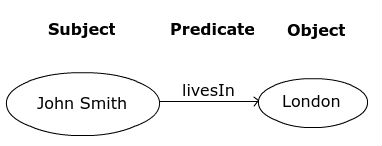
\includegraphics[scale=0.65]{gambar/rdfinstance.jpg}
			\caption{Sebuah representasi RDF untuk sebuah informasi}
			\label{fig:rdfinstance}
	\end{figure}

	Ide sederhana dari unit informasi ini adalah bahwa unit informasi tersebut dapat dinyatakan dalam berbagai format yang dengan mudah di mengerti oleh mesin. \emph{RDFS (RDF Schema)} digunakan untuk menggambarkan properti dan kelas dari sebuah dokumen \emph{RDF}. Pewujudan dari triple pada gambar \ref{fig:rdfinstance} dapat dinyatakan dalam XML dan JSON berikut:

	\begin{figure}[H]
		\centering
			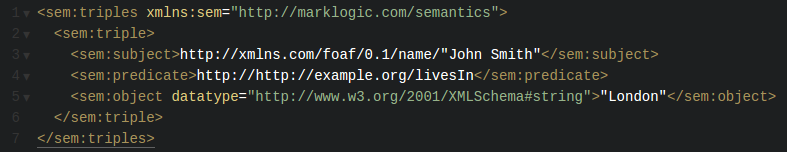
\includegraphics[scale=0.5]{gambar/rdfinstancexml.png}
			\caption{RDF dalam format XML}
			\label{fig:rdfinstancexml}
	\end{figure}

	\begin{figure}[H]
		\centering
			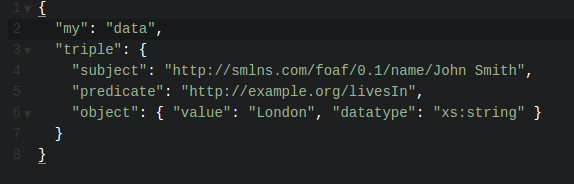
\includegraphics[scale=0.5]{gambar/rdfinstancejson.png}
			\caption{RDF dalam format JSON}
			\label{fig:rdfinstancejson}
	\end{figure}

\section{\emph{Web Ontology Language (OWL)}}
	\emph{Web Ontology Language (OWL)} atau Ontologi adalah sebuah standar dari \emph{W3C} untuk membantu perkembangan Web Semantik. \emph{OWL} memberikan interpretasi mesin yang lebih besar dengan memberikan kosa kata tambahan beserta semantik lainnya. \emph{OWL} menambahkan lebih banyak kosakata untuk menggambarkan \emph{RDFS (RDF Schema)}. Konsep ini merupakan ide dasar dibalik peningkatan kemampuan mesin untuk dapat mengerti dengan menggunakan \emph{OWL}

	\emph{OWL} dikategorikan menjadi tiga sub bahasa agar sesuai dengan kebutuhan pengguna: 

	\vspace{-0.5cm}

	\begin{enumerate}[a.]
	\begin{singlespace}
	\itemsep0em
		\item \emph{OWL DL} -- \emph{DL} merupakan singkatan dari \emph{Description Logics}, yang merupakan salah satu bidang dasar untuk penciptaan \emph{OWL}. \emph{OWL DL} diperuntukkan bagi pengguna yang ingin mencapai ekspresivitas penuh suatu topik sambil memastikan bahwa perhitungan akan selesai pada waktu yang terbatas,
		\item \emph{OWL Lite} -- Sebuah sub bahasa sederhana yang menyediakan hirarki dan batasan klasifikasi. Kardinalitas hanya bisa memiliki nilai 0 atau 1, sehingga membatasi dan mengurangi kompleksitas hubungan,
		\item \emph{OWL Full} -- \emph{OWL Full} ditujukan untuk pengguna yang perlu melintasi seluruh hierarki subjek ke akarnya dan bahkan \emph{metadata} dari \emph{root}. \emph{OWL Full} tidak memiliki jaminan komputasi karena cukup dapat dimengerti bahwa proses ini bisa sangat kompleks. Namun, \emph{OWL Full} mendorong untuk menciptakan semua kemungkinan makna kelas \emph{RDF}.
	\end{singlespace}
	\end{enumerate}

\section{Ontologi}
Ontologi tidak memiliki definisi yang diterima secara formal. Namun, kosakata dan ontologi sering digunakan dengan makna yang sama. Ontologi dapat didefinisikan sebagai seperangkat \emph{URI} yang membentuk makna untuk topik tertentu. Unit yang membentuk ontologi adalah satu set \emph{RDF} bersama dengan \emph{OWL}. Ada berbagai ontologi yang telah diciptakan dan sering digunakan. Namun sebagian besar ontologi diciptakan oleh manusia dan mesin memiliki sedikit sekali kontribusi dalam hal ini.

Contoh beberapa ontologi: \emph{Dublin Core} -- Mereka memiliki ontologi untuk metadata data. Kumpulan ontologi mereka mencakup kelas, properti, skema pengkodean kosa kata, skema pengkodean sintaks dan koleksi. Semua dari mereka memiliki beberapa set \emph{RDF} yang menjelaskan data tentangnya. \emph{Dbpedia} - "Ini adalah upaya bersama komunitas untuk mengambil informasi terstruktur dari \emph{Wikipedia} dan membuat informasi ini tersedia di Web. \emph{Dbpedia} memungkinkan Anda untuk mengajukan pertanyaan yang canggih terhadap Wikipedia, dan untuk menghubungkan kumpulan data yang berbeda pada data Web ke Wikipedia. Lebih jauh lagi, dbpedia mungkin mengilhami mekanisme baru untuk navigasi, kaitan, dan peningkatan ensiklopedia itu sendiri." Kutipan di atas adalah deskripsi resmi \emph{Dbpedia} dari pembuatnya. Bisa dikatakan bahwa \emph{Dbpedia} adalah versi Web Semantik dari \emph{Wikipedia}. Ontologi \emph{Dbpedia} sangat besar dan memiliki 4,2 juta objek yang mencakup hal-hal, orang, tempat, pekerjaan, organisasi, dan spesies. Jumlah data yang besar ini disusun menggunakan \emph{RDF} dan \emph{OWL}. Beberapa di antaranya terkait dengan sumber data terkait lainnya yang mengubah Dbpedia menjadi inti dari jaringan data seperti yang telah disebutkan.

Ada berbagai contoh ontologi seperti \emph{FOAF}, \emph{Good Relations}, \emph{Music Ontology} dll. Sekarang semua ontologi ini perlu disimpan di suatu tempat dan untuk tujuan itu kita memiliki \emph{Triple Stores}.

\section{\emph{Triple Stores}}
\emph{Triple Store} adalah jenis khusus \emph{database} untuk menyimpan dan mengambil \emph{triples}. \emph{Triple stores} dibuat khusus untuk \emph{Semantic Web} dan \emph{Linked Data}. Serupa dengan \emph{database} yang lain \emph{triple store} mengambil informasi melalui bahasa \emph{query}. \emph{Triple Store} juga memiliki kemampuan untuk mengimpor dan mengekspor informasi yang dibutuhkan dalam format \emph{RDF}.

Ada banyak varian yang berbeda dari Triple Stores, beberapa di antaranya diciptakan dari nol dan beberapa di antaranya dibangun di atas database \emph{SQL} dan \emph{NoSQL} yang telah ada. \emph{Triple Store} sering juga disebut sebagai \emph{RDF Store}. Beberapa contoh \emph{Triple Stores} adalah:

\begin{enumerate}[a.]
	\item \emph{Virtuoso} -- adalah middleware yang mendukung Sistem Manajemen Database Relasi Tradisional (RDBMS) dan juga memiliki dukungan khusus untuk penyimpanan dan pengambilan dokumen \emph{RDF}. \emph{Virtuoso} mendukung beberapa protokol dan menggunakan proses \emph{multi-threaded} tunggal. Hal ini juga dikenal sebagai \emph{Openlink Virtuoso}. Virtuoso menyediakan \emph{SPARQL Endpoint} seperti semua \emph{Triple Store} lainnya. \emph{Virtuoso} terkenal dengan kinerjanya dalam mengolah \emph{dataset} besar. Misalnya, \emph{Dbpedia} di-host di \emph{Virtuoso Triple Store}.
	\item \emph{Fuseki} -- adalah proyek turunan dari \emph{Apache Jena}. \emph{Fuseki} menyediakan server \emph{RDF} yang bisa menjadi \emph{Triple Store}, yang dapat dikelola melalui protokol \emph{REST}. \emph{Fuseki} bisa berjalan sebagai service pada mesin remote, \emph{WAR (Java Web Archieve)} atau sebagai \emph{server standalone}. \emph{Fuseki} mendukung \emph{SPARQL 1.1} dan juga menambahkan dukungan logging untuk memantau apa yang terjadi di \emph{triple store}. Versi terbaru \emph{Fuseki v2}, memberikan fitur keamanan melalui \emph{Apache Shiro}. \emph{Apache Shiro} menambahkan kriptografi dan manajemen sesi ke \emph{Fuseki}. 
\end{enumerate}

\section{\emph{SPARQL}}
\emph{SPARQL} adalah standar \emph{W3C} lain dalam kategori \emph{Semantic Web}. \emph{SPARQL} adalah bahasa query yang mirip dengan \emph{Structured Query Language (SQL)} untuk \emph{Relational Database Management Systems (RDBMS)}. \emph{SPARQL} digunakan untuk melakukan \emph{query} dokumen \emph{RDF}. Hal ini memungkinkan representasi grafik dari dokumen \emph{RDF}. \emph{Query SPARQL} bisa menghasilkan set grafik. Hasilnya bisa berupa nilai literal ataupun \emph{URI}. Kemampuan untuk mengambil literal atau bahkan mengubah \emph{URI} menjadi label memberikan cara langsung dan mudah bagi aplikasi untuk menggunakan hasil \emph{query}.

\section{Jadwal Kegiatan}

	% Please remember to add \use{multirow} to your document preamble in order to suppor multirow cells
		\begin{table}[H]
		\centering
		\caption{Jadwal Penelitian.}
		\label{jadwal}
		\begin{tabular}{|c|l|l|l|l|l|l|l|}
		\hline
		\multirow{2}{*}{No} & \multirow{2}{*}{Keterangan} & \multicolumn{6}{c|}{Bulan}                                                                                                                          \\ \cline{3-8} 
		                    &                             & 1 & 2 & 3 & 4 & 5 & 6 \\ \hline
		1                   & Studi literatur                                  &\cellcolor{gray} &\cellcolor{gray}&                        &                        &                        &                         \\ \hline
		2                   & Desain                                           &                        &\cellcolor{gray}&\cellcolor{gray}&                        &                        &                         \\ \hline
		3                   & Pembelian bahan                                  &                        &                        &\cellcolor{gray}&                        &                        &                         \\ \hline
		4                   & Pembuatan prototipe                              &                        &                        &\cellcolor{gray}&\cellcolor{gray}&\cellcolor{gray}&                         \\ \hline
		5                   & Uji coba dan perbaikan                           &                        &                        &                        &\cellcolor{gray}&\cellcolor{gray}&                         \\ \hline
		6                   & Penulisan skripsi                                &                        &                        &                        &                        &                        &\cellcolor{gray}\\ \hline
		\end{tabular}
		\end{table}
	
% Baris ini digunakan untuk membantu dalam melakukan sitasi
% Karena diapit dengan comment, maka baris ini akan diabaikan
% oleh compiler LaTeX.
\begin{comment}
\bibliography{daftar-pustaka}
\end{comment}
